% Created 2019-09-29 Sun 13:49
% Intended LaTeX compiler: pdflatex
\documentclass[a4paper, 11pt]{extarticle}
             \usepackage[utf8]{inputenc}
\usepackage[left=2cm, right=2cm, bottom=2.5cm, top=2.5cm]{geometry}
% Paquetes de matemáticas
\usepackage{amsmath, amsfonts, amssymb, commath}
\usepackage{tikz}
\newcommand{\tikzcircle}[2][red,fill=red]{\tikz[baseline=-0.5ex]\draw[#1,radius=#2] (0,0) circle ;}%
% Ajustes de idioma, gráficos, etc
\usepackage{adjustbox}
\usepackage{float}
\usepackage{hyperref}
\usepackage{graphicx}
\usepackage{gensymb}
\usepackage[spanish, english]{babel}
\usepackage{tikz}
\usepackage{multicol}
\usepackage{listings}
\usepackage{enumitem}
\setlist{nolistsep}
\usepackage{booktabs}
\usepackage{xcolor}
\usepackage{wrapfig}
%Fuentes.
% Alegreya tiene este toque antiguo con serifa, y la tipografía de las ecuaciones es también interesante.
% Gillius no tiene serifa, y también es equilibrada.
\usepackage[T1]{fontenc}
%\usepackage[default]{gillius}
\usepackage{newpxtext, newpxmath}
% Paquete para añadir Creative Commons al final del documento
\usepackage[
type={CC},
modifier={by-nc-nd},
version={3.0},
]{doclicense}
% Propiedades de párrafo
\setlength{\parindent}{0em}
\setlength{\parskip}{1.1em}
\renewcommand{\baselinestretch}{1.05}
\setlength\itemsep{0em}
% Definición de comandos. Muchos de ellos han surgido para Geometría, aunque se
% irá actualizando la lista. POSIBLEMENTE LO INTRODUZCA COMO COMANDOS DE ORG
\newcommand{\m}{\text{medio}}
\newcommand{\iso}{\text{Isom}}
% Para incluir mathcal en las ecuaciones. El /mathcal para Alegreya es el viejo
% y floritural estilo que odio.
\usepackage{calrsfs}
\DeclareMathAlphabet{\pazocal}{OMS}{zplm}{m}{n}
% Definición de colores agradables a la vista
\definecolor{azul}{HTML}{107896}
\definecolor{naranja}{HTML}{C2571A}
\definecolor{rojo}{HTML}{9A2617}
\definecolor{amarillo}{HTML}{BCA136}
\definecolor{verde}{HTML}{829356}
\definecolor{gris}{HTML}{909090}
\definecolor{rosa}{HTML}{F9A7B0}
\definecolor{amarillochillon}{HTML}{FBB117}
% Definición de comandos para teoremas, etc. El comando también incluye
% como argumento un texto, del estilo Teorema 3.5
\newcommand{\axioma}[1]{\textcolor{naranja}{\textbf{Axioma #1}}}
\newcommand{\tma}[1]{\textcolor{rojo}{\textbf{Teorema #1}}}
\newcommand{\propo}[1]{\textcolor{rojo}{\textbf{Proposición #1}}}
\newcommand{\defi}[1]{\textcolor{azul}{\textbf{Definición #1}}}
\newcommand{\obs}[1]{\textcolor{verde}{\textbf{Observación #1}}}
\newcommand{\ejem}[1]{\textcolor{verde}{\textbf{Ejemplo #1}}}
\newcommand{\ej}[1]{\textcolor{amarillo}{\textbf{Ejercicio #1}}}
\newcommand{\lema}[1]{\textcolor{rosa}{\textbf{Lema #1}}}
\newcommand{\cor}[1]{\textcolor{rosa}{\textbf{Corolario #1}}}
% La demostración es igual pero va con una letra más pequeña y en gris.
\newcommand{\dem}[1]{\textcolor{gris}{\small{Demostración. #1}}}
% Esto pone un triangulito de peligro para cuando algo es importante.
\newcommand{\importante}{\tikzcircle[amarillo, fill=amarillo]{4pt}\,}
% Para usar columnas emplea este trozo de código
% \begin{multicols*}{2}
% [\section{Axiomas para la geometría euclidiana plana}]
% 	\axioma{P1} Si tenemos el conjunto $\P$, denominado \textbf{plano}, y la aplicación $d:\P \times \P \rightarrow \R$ llamada \textbf{distancia}, entonces$(\P, d)$ es un espacio métrico.

\defi{2.2} Una \textbf{recta} $r \subset \P$ satisface
\begin{itemizex}
	\item $r$ contiene al menos dos puntos.
	\item Para toda terna de puntos $A, B, C$, están alineados si están en $r$.
\end{itemizex}

\axioma{P2} $\P$ contiene al menos tres puntos no alineados; y por dos puntos distintos, $A$ y $B$ de $\P$ pasa una recta, $r_{AB}$.

\defi{2.6} / \tma{2.7} Dos rectas se cortan si sólo tienen un punto en común, y si no tienen ningún punto en común, entonces se denominan \textbf{paralelas}, y se denota por $a \parallel b$. Dos rectas, o se cortan o son paralelas.

\importante\axioma{P3} Para toda recta $r \subset \P$ existe una biyección $\gamma: r \rightarrow \R$ tal que $|\gamma(X) - \gamma(Y)| = |x - y| = d(X, Y) \;\; \forall \;\; X,Y \in r$ 

\obs{2.8} Si $A, B \in r$ son distintos, entonces existe un punto $M\in r: d(A,M) = d(M,B)$ que denotamos por $\m[A,B]$ y se llama \textbf{punto medio}. Asimismo sólo existe un punto $B \in r$ tal que $B = \m[A, M]$.

\obs{2.9} Si $r$ es una recta y $P \in r$, entonces $r$ se puede dividir en dos \textbf{semirrectas}, que son los conjuntos $\{X \in r \; | \; \gamma(X) > \gamma(P)\}$ y $\{X \in r \; | \; \gamma(X) < \gamma(P)\}$.

\axioma{P4} Para toda recta $r \subset \P$ hay dos subconjuntos $H^1$ y $H^2$, denominados \textbf{semiplanos} de $r$, que verifican:
\begin{itemizex}
	\item $H^1 \cup H^2 = \P-r$
	\item Si $X,Y \in H^i$ entonces $[X,Y] \subset H^i$
	\item Si $X \in H^1$ y $Y \in H^2$ entonces $[X,Y] \cap r \neq \emptyset$.
\end{itemizex}

\defi{2.15} Sean $P, Q, R$ no alineados, entonces el triángulo $\triangle\{P,Q,R\}$, o $\triangle PQR$ está formado por los segmentos $[P,Q]$, $[Q,R]$, $[P,R]$, llamados lados, y los vértices $P,Q, R$.

\tma{2.16 [Axioma de Pasch]a} Dado un triángulo $\triangle PQR$ y una recta $r$; si $r$ corta a $[P,Q]$, entonces o corta a $[P,R]$ o a $[Q, R]$.

\defi{2.17 = 1.5} Una \textbf{isometría} en $\P$ es una biyección $g: \P \rightarrow \P$ que cumple que $d(g(X), g(Y)) = d(X,Y) \;\;\forall\;\; X,Y \in \P$.

\tma{2.18} Si $A,B \in \P$ y $g \in \iso(\P)$ entonces $g([A,B]) = [g(A), g(B)]$ y $g(r_{AB}) = r_{g(A)g(B)}$ 

\axioma{P5} Si $A_1, A_2 \in \P$ y $B_1, B_2 \in \P$ son dos pares de puntos que cumplen $d(A_1,A_2) = d(B_1,B_2)$ entonces existe $g \in \iso(\P)$ tal que $g(A_i) = B_i$. Se dice que esos pares de puntos son \textbf{congruentes}.

\axioma{P6} Para toda recta $r$ existe una isometría $\sigma$ llamada \textbf{reflexión} tal que  
\begin{itemizex}
	\item $\sigma(X) = X\iff X \in r$
	\item $\sigma \circ \sigma = \text{Id}$
\end{itemizex}


\defi{2.23} / \tma{2.25} / \cor{2.30} Una recta $l$ es \textbf{ortogonal} a $r$ si para todo $S \in l$ y para todo par de puntos $A, B$ que cumple que $M = \m[A,B]$, de modo que $l \cap r = M$, entonces se da que $d(A,S) = d(S,B)$. Se denota $l \perp_M r$. En estas condiciones, $l = \{X \in \P \; | \; d(S,A) = d(S,B)\}$, se denomina \textbf{mediatriz} de $[A,B]$. 

\begin{figure}[H]
	\centering
	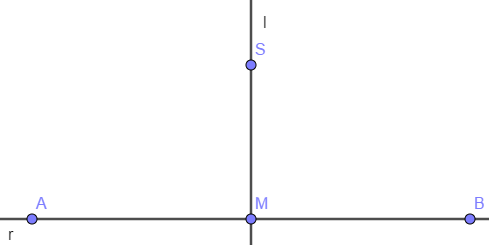
\includegraphics[width=7cm]{figuras/2-23.png}
	\vspace{-1em}
\end{figure}

\lema{2.21} Si $\sigma_r$ entonces, para todo $X$, $\m[X, \sigma_r(X)] \in r$.

\obs{2.24} Si $l \perp r$ y $g \in \iso(\P)$ entonces $g(l) \perp g(r)$.

\importante\tma{2.26} Si $l, r \subset \P$ cortan en $M$ y $\sigma_l, \sigma_r$ son dos reflexiones de $l$ y $r$, entonces se cumple que $l \perp_M r \iff r \perp_M l \iff \sigma_r(l) = l \iff \sigma_l(r) = r$.

\importante\tma{2.27 / 2.29} Para toda recta $r$ y todo punto $S \in \P - r$, existe una recta $l$ ortogonal a $r$, que pasa por $S$. Si $r$ es una recta, y $M \in r$, entonces existe $l$ tal que $l \perp_M r$.

\axioma{P7} Para toda recta $r$ y todo punto $P$ existe sólo una recta \textbf{paralela} a $r$ que pase por $P$.

\tma{2.31 / 2.33} Si $a \perp l$ y $b \perp l$ entonces $a \parallel b$. Sean $a \parallel b$. Entonces, para todo $A \in a$, la única recta $l \perp_A a$ también es ortogonal a $b$.

\tma{2.32} Las rectas parallelas forman una relación de equivalencia.
\begin{itemizex}
	\item Reflexividad: $a\parallel a$
	\item Simetría: $a \parallel b \rightarrow b \parallel a$
	\item Transitividad  $a \parallel b $ y  $b \parallel c \rightarrow a \parallel c$
\end{itemizex}

\ej{2.6} Sean $A,B \in r$, $A \neq B$. Para todo $t$, existe un único $P_t\in r$ que cumple $d(P_t,A) = \abs{t}$ y $d(P_t, B) = \abs{t-d(A,B)}$. En definitiva, la posición de $P_t$ está sólamente determinada por las distancias $d(A, P_t)$ y $d(P_t, B)$.
	 
	 
	 
	 
	 
	 
	 \end{multicols*}\pagebreak
% multicols* obliga a terminar una columna antes de empezar la siguiente.
\DeclareMathAlphabet{\pazocal}{OMS}{zplm}{m}{n}
\let\mathcal\pazocal
\usepackage{fancyhdr}
\pagestyle{fancy}
\lhead{Alex Martínez Ascensión}
\chead{}
\rhead{\today}
\date{}
\title{\Huge\vspace{-1em}Estructuras algebráicas}
\hypersetup{
 pdfauthor={},
 pdftitle={\Huge\vspace{-1em}Estructuras algebráicas},
 pdfkeywords={},
 pdfsubject={},
 pdfcreator={Emacs 26.2 (Org mode 9.2.5)}, 
 pdflang={English}}
\begin{document}

\maketitle
\vspace{-8em}

\section{Generalidades y teorema de Lagrange}
\label{sec:org2ef7eb2}
\subsection{Grupos}
\label{sec:org6a36c99}
\defi{1.1} Un grupo es un conjunto no vacío \(G\) en el que se define una 
operación binaria \(G \times G \rightarrow G\;;\; (a,b) \mapsto ab\) que cumple (1) \textbf{asociatividad}
(\((ab)c = a(bc)\)), (2) \textbf{existencia de elemento neutro} \(u \in G\;;\;ua=a=au\)
y (3) \textbf{existencia de elemento inverso} \(a,x \in G \;;\; ax = u = xa\). Tanto \(u\) como \(a\) 
son únicos. Para la suma \(u = 0, a=-x\) y para el producto \(u = 1, a = x^{-1}\).

Otras propiedades inmediatas de los grupos son (1) \textbf{simplificación}:
 \(ab=ac \iff b=c\); \(ba = ca \iff b=c\); (2) \textbf{asociatividad generalizada}:
 \((a_1 \cdots a_k)(a_{k+1} \cdots a_n ) =
(a_1 \cdots a_l)(a_{l+1} \cdots a_n)\) 
, (3) \textbf{inverso de un producto}: \((a_1 \cdots a_n)^{-1}  = a_n^{-1} \cdots
a_1^{-1}\).

\defi{1.2} Un \textbf{grupo simétrico} \(S_n\) es el conjunto de biyecciones de un
conjunto \(X\) con \(n\) elementos. Se cumple que \(\text{card}(S_n) = n!\). Otros ejemplos de 
grupos son \(GL_n(\mathbb{R})\), el grupo de matrices no
singulares para la operación producto; o \(D_n\) es el conjunto de biyecciones
que conserva la distancia en un polígono de \(n\) lados. 

\defi{1.3} Un grupo es \textbf{abeliano} si \(ab = ba\;\; \forall a,b \in G\).
Todo grupo con dos elementos es abeliano, pues \(aa = aa; uu=uu; ua=a=au\);
pero para \(n \ge 3\), \(S_n\) no puede ser abeliano. \(GL_n; n \ge 2\),
ni \(D_n; n \ge 3\) son abelianos.

\propo{1.4} (1) Si \(x^2 = 1 \; \forall x \in G\), entonces \(G\) es
abeliano; (2) si \((ab)^2=a^2b^2\) entonces \(G\) es abeliano.

\dem{ (1) Para cada $x,\; x \cdot x = 1 \iff x = x^{-1}$, luego si $a,b \in G$ 
entonces $a = a^{-1}; b=b^{-1}$x y si $c = ab$ entonces 
 $ab = c =c^{-1} = (ab)^{-1} = b^{-1}a^{-1} = ba$. (2) Dados $a,b \in G$,  se tiene
 que $a(ba)b = (ab)^2 = a^2b^2 = a(ab)b$ y, por simplificación, $ab = ba$.  }


\defi{1.5} Si \(G,G'\) son dos grupos con operaciones
\(G \times G \rightarrow G: (a,b) \mapsto ab \quad;\quad G' \times G' \rightarrow G': (a', b') \mapsto a'b'\)
 el \textbf{producto cartesiano} \(G'' = G \times G''\) es un grupo con operación 
\(G'' \times G'' \rightarrow G'': ((a, a'), (b, b')) = (ab, a'b')\). La asociatividad se mantiene, 
y se ve que \(1_{G''} = (1_G, 1_{G'})\).
Además, si \(G, G'\) son abelianos, \(G''\) también lo es. Se dice que \(G_1 \times \cdots \times G_r\) es el \textbf{producto directo}.

\subsection{Subgrupos}
\label{sec:orgc6d76e5}
\defi{1.6} Un subconjunto no vacío \(H \subset G\) es un \textbf{subgrupo} de \(G\) si es un grupo con la misma operación que \(G\).
\textbf{EN ALGUNOS SITIOS \(H \subset G\) INDICA QUE \(H\) ES SUBGRUPO DE \(G\).}
Se puede ver que el elemento neutro de \(H\) es \(1_G\), y que si \(x \in H;
x^{-1} \in H\). Para que (1) \(H\) sea subgrupo de \(G\) se tiene que cumplir que
(2) si \(x,y \in H\), entonces \(x y^{-1} \in H\).

\(\{ 1_G \}\) y \(G\) son subgrupos de \(G\). El resto de subgrupos se
llaman \textbf{subgrupos propios} de \(G\). Por ejemplo, \(m \mathbb{Z} = \{ mx \;|\;
x,m \in \mathbb{Z}; 
\}\) es un subgrupo de \(\mathbb{Z}\). 

\defi{1.8.3} Se denomina a \(\langle S \rangle\) al \textbf{subgrupo generado} por \(S\). 


\(\langle S \rangle  = \left\{ s_1^{h_1} \cdots s_n^{h_n} \;|\; n \in \mathbb{N} , s_i \in S, h_i \in \mathbb{Z}
 , 1 \le i \le n
 \right\}\). Esto se puede simplificar como


\(\langle S \rangle  = \left\{ x_1 \cdots x_m \;|\; m \in \mathbb{N} , x_i \in S,  1 \le i \le m
 \right\}\). Es decir, es el conjunto de todos 
 los elementos de \(S\) combinados con operación binaria. Si \(\mathcal{F}_S\) es la
familia de los subgrupos de \(G\) que contienen a \(S\), entonces se cumple
que \(\langle S \rangle = \bigcap_{H \in \mathcal{F}_S}^{} H\).

Un caso particular es cuando \(S = \{ a \}\). En tal caso es el \textbf{subgrupo
generado por a}, \(\langle a \rangle = \{ a^k \;|\; k \in \mathbb{Z}\}\). Un subconjunto \(S \subset G\) se llama \textbf{generador de \(G\)} si \(G = \langle S \rangle\). Es cierto que
\(\langle G \rangle = G\). Si \(S\) es finito, entonces se dice que \(G\) es \textbf{finitamente generado}.

\defi{1.8.4} Si \(H\) es subgrupo de \(G\), se llama \textbf{centralizador de \(H\) en \(G\)} a \(C_G(H) = \{ x \in G \;|\; ax=xa \; \forall a \in H \}\).
El
centralizador de \(G\) en \(G\), llamado \textbf{centro de \(G\)} es el caso \(Z(G) = \{ x \in G \;|\; xa = ax \; \forall a \in G \}\). Se ve que \(C_G(H)\) es un
subgrupo de \(G\).

\defi{1.8.5}  Si \(S \subset G\) y \(a \in G\), se llama \textbf{conjugado de \(S\) por \(a\)} al conjunto 
\(S^a = \{ a^{-1}xa \;|\; x \in S \}\)

\defi{1.8.6} Si \(S \subset G\), se llama \textbf{normalizador de \(S\) en \(G\)} al conjunto 
\(N_G(S) = \{ a \in G \;|\; S^a = S \}\).
El normalizador de \(S\) es un subgrupo de \(G\) porque si \(a,b \in N_G(S)\), entonces \(S^{ab^{-1}} = (S^a)^{b^{-1}} = S^{b^{-1}} = (S^b)^{b^{-1}} =
S^{bb^{-1}} = S\)

\defi{1.8.8} Dados dos subgrupos \(K,H\) de \(G\), se define 
\(HK = \{ hk \;|\; h \in H, k \in K \}\).
Para que \(HK\) sea un subgrupo de \(G\) entonces \(HK = KH\).
Si \(H \subset K, HK = K = KH\).

\subsection{Orden de un grupo}
\label{sec:org181dd8f}
\defi{1.9} El \textbf{orden} de un subgrupo finito \(H \subset G\) es el número de elementos que tiene. Se denota por \(o(H)\). Un elemento \(a \in G\) es \textbf{de torsión} si \(\langle a \rangle\) es finito. En tal caso el orden
es \(o(a)\).

\propo{1.10} Sea \(G\) un grupo y \(a \in G\) de torsión. Entonces se cumple
que 
\begin{itemize}
\item Existe \(k \ge 1\) tal que \(a^k=1\)
\item \(o(a)\) es el menor número tal que \(a^n=1\)
\item Si \(n=o(a), \langle a \rangle = \{ 1, a, \cdots, a^{n-1} \}\)
\item \(a^k=1\) sii \(k\) es múltiplo de \(n\)
\item \(o(a^{-1}) = o(a)\)
\item Si \(x = a^k\) y \(n=o(a)\), entonces \(o(x) = \frac{n}{mcd(n,k)}\)
\item Si \(b \in G\) es de torsion y \(ab=ba\) entonces \(o(ab)\) es divisor de
\(mcm(o(a),o(b))\). Si \(o(a), o(b)\) son primos entre si, \(o(ab) =
  o(a)o(b)\)
\item \(o(ab) = o(ba)\)
\end{itemize}

\subsection{Índice de un subgrupo}
\label{sec:org2a1e17e}
\defi{1.2}/\obs{1.12.6/7} Sea \(G\) un grupo y \(H \subset G\).  Sean \(R^H, R_H\) las relaciones de equivalencia en \(G\):
\[ xR_H y \iff xy^{-1} \in H \]
\[ xR^H y \iff x^{-1}y \in H \]
Además, se definen \(Hx = \{ hx \;|\; h \in H \}; xH = \{ xh \;|\; h \in H \}\).
Se cumple que si \(x,y \in G\), y \(yR_H x\) entonces \(yx^{-1} = h \in H\) y,
por tanto, \(y = hx \in Hx\).

Además, las aplicaciones \(H \rightarrow Hx: h \mapsto hx\) y su equivalente en \(xH\) son
biyectivas. Es importante que pese a existir una biyeccíón entre
 \(Hx\) y \(xH\), \textbf{no siempre \(Hx\) y \(xH\) son iguales}.

\propo{1.12.3} La aplicación entre conjuntos cocientes
 \(G/R_H \rightarrow G/R^H: Hx \rightarrow x^{-1}H\) es biyectiva.

\defi{1.12.4} \(H \subset G\) es un subgrupo de \textbf{índice infinito} si \(G/R_H\) es
un conjunto infinito. Por otra parte, el índice de \(H\) en \(G\), \([G:H]\) es
 el número de elementos de \(G/R_H\).

\propo{1.12.8 (T de Lagrange)} Sea \(H \subset G\) un subgrupo. Se cumple que 
si \(G\) es finito, entonces \(o(H)\) es
finito, \(H\) tiene índice finito en \(G\) y \(o(G) = o(H) \cdot [G:H]\).

\cor{1.12.9} Si \(H,K\) son subgrupos finitos de \(G\), \(o(H) = m\), \(o(K) = n\), 
entonces \(o(H \cap K) = 1 \iff H \cap K = \{ 1_G \}\)

\propo{1.12.10 (F de transitividad del índice)} Sean \(H,K\) 
subgrupos de \(G\). Si \(H\) es subgrupo de \(K\), y los indices entre subgrupos, y con G,
son finitos, entonces se cumple \([G:H] = [G:H][H:K]\)

\propo{1.12.11} Sean \(H,K\) subgrupos de \(G\), finito. Entonces
\[ card(HK) = \frac{o(H)o(K)}{o(H \cap K)} \]


\defi{1.15} / \obs{1.15.4} Un grupo \(G\) se llama \textbf{cíclico} si existe
 \(a \in G\) tal que \(G
= \langle a \rangle\). Si \(o(a) = p\), primo, el grupo es cíclico.

\propo{1.16 / 1.17} Sea \(G\) cíclico y \(n = o(G)\), para cada divisor \(m\) de
\(n\)
existe un único subgrupo de \(G\) de orden \(m\), y ese subgrupo es cíclico.
Además, todo subgrupo de un grupo cíclico [finito o no] es cíclico.

\defi{1.18} Sea \(G\) finitamente generado. Un sistema generador \(S\) se
llama \textbf{minimal} si cualquier subconjunto de \(G\) con menos elemenos que \(S\)
no es generador de \(G\).

\propo{1.19} Sea \(G\) finito de orden \(n\) y \(S = \{ x_1, \cdots, x_p \}\)
un
sistema generador minimal de \(G\). Entonces \(2^p \le n\).

\dem{ Llamamos \( S_i = \{ x_1, \cdots, x_i \}, \; 1 \le i \le p \); y \( H_i = \langle S_i \rangle \). 
Evidentemente, \( H_i \subset H_{i+1}
\). Por ele teorema de Lagrange y la fórmula de la transitividad del índice,
\[ [G:H_1] = [H_P:H_1] = [H_P:H_{P-1}][H_{P-1}:H_{P-2}]\cdots[H_2:H_1] \]
Además, 
\[ [H_{i+1}:H_i] = \frac{o(H_{i+1})}{o(H_i)} > 1 \iff
[H_{i+1}:H_i] \ge 2 \]
pues los índices son enteros.
Por tanto, \( [G:H_1] \ge 2^{p-1} \), y como \( o(H_1) \ge 2 \), entonces,
\( o(G) = o(H_1)[G:H_1] \ge 2^p \)
}

\pagebreak
\textcolor{gris}{\textit{Page intentionally left in blank}}
\newpage
\pagebreak


\section{Subgrupos normales, homomorfismos, teorema de estructura de grupos abelianos finitos}
\label{sec:org57b4ab6}
 \propo{2.1} Sea \(G\) un grupo y \(H\) un subgrupo. \(H\) es un subgrupo
\textbf{normal} (\textbf{LO DEFINO AQUÍ COMO} \(\subset_N\)) si se cumplen las condiciones equivalentes:
\begin{enumerate}
\item Para todo \(a  \in G\), \(aH = Ha\)
\item Para todo \(a \in G\), \(H = H^a\)
\item Para todo \(a,b \in G\), \(ab \in H \iff ba \in H\), luego \(H\) es
abeliano.
\end{enumerate}

\obs{2.2.1} Si \(H\) es normal, entonces \(R^H = R_H\), y \(G/R_H\) se
escribe \(G/H\).

\obs{2.2.4/2.2.5} Si \(H\) es un subgrupo de \(G\), y \([G:H] = 2\), \(H\) es subgrupo normal de \(G\). Asimismo, los subgrupos \(\{ 1_G \}, G\) son 
normales.

\defi{2.2.14} Un grupo \(G\) es \textbf{simple} si los únicos subgrupos son  \(\{ 1_G
\}, G\). Si \(o(G)\) es primo \(p\), por el teorema de Lagrange, los únicos
subgrupos son \(\{ 1_G \}, G\), luego \(G\) es simple.

\propo{2.2.8} Todo subgrupo \(H \subset Z(G) = \{ a \in G \;|\; ag = ga\;
\forall g \in
H\}\) es subgrupo normal de \(G\).

\propo{2.2.10} Sea \(H\) subgrupo de \(G\).
\begin{enumerate}
\item \(H\) es subgrupo de \(N_G(H) = \{ a \in G \;|\; H = H^a \}\).
\item \(H \subset_N
   N_G(H)\).
\item Si \(H \subset K \subset G\) y \(H \subset_N
   K\),
entonces \(K \subset N_G(H)\).
\end{enumerate}

\defi{2.2.11} Si \(H,K\) son subgrupos de \(G\), \(K\) es un \textbf{subgrupo
conjugado} de \(H\) si existe \(a \in G\) tal que \(K = H^a\). Como la
relación es recíproca, se dice que \(K\) y \(H\) son conjugados.

\propo{2.2.11} 
\begin{itemize}
\item Si \(\Sigma\) es la familia de conjugados de \(H\) y \(N = N_G(H)\), la aplicación \(\phi: G/R_N \rightarrow \Sigma: Na \rightarrow H^a\) es biyectiva.
\item Si \(N\) tiene índice finito en \(G\), el número de conjugados con \(H\) es \([G:N]\).
\end{itemize}

\propo{2.2.13} Si \(A \subset_N G\), \(H \subset K \subset G\), y \(H \subset_N K\), entonces \(AH \subset_N AK\).

\importante La normalidad no es transitiva, es decir, si \(H \subset_N
K \subset_N G\), no siempre es cierto que \(H \subset_N G\).

\defi{2.2.16}/\obs{2.2.16.1} Si \(H \subset G\), se llama corazón de \(H\) a \[
\heartsuit(H) =  K(H) = \bigcap_{a \in G}^{} H^a \]

Si \(N \subset_N H\) entonces \(N \subset K(H)\), pues para cada \(a \in G\): \(N = N^a
\subset H^a\), luego \(N = N^a \subset \cap_{a \in G} H^a = K(H)\)

\propo{2.2.17 (T de Poincaré)} Si \(G\) posee un subgrupo de índice
finito, también posee un subgrupo normal de índice finito.

\subsection{Grupos cocientes}
\label{sec:org160e593}
\propo{2.3} El grupo cociente \(G/H\) de \(H \subset_N G\) tiene estructura de grupo con la operación:
\begin{align*}
 &\; G/H \times G/H  
 \longrightarrow G/H 
 \\
$       &\; (aH, bH) \longmapsto     abH 
\end{align*}

El elemento neutro del grupo cociente es \(H\), y el inverso de \(aH\) es \((aH)^{-1} = a^{-1}H\).

\obs{2.3.1} Si \(H \subset_N K \subset G\) (entonces \(H \subset_N G\)), el
grupo cociente \(K/H \subset G/H\),  ya que si \(aH,bH \in K/H, a,b \in K\), entonces \((aH)(bH)^{-1} =
(aH)(b^{-1}H) = ab^{-1}H \in K/H\), ya que como \(K \subset G
, ab^{-1} \in K\)

\obs{2.3.1.1} \(K \subset_N G \iff K/H \subset_N G/H\)

\ejem{2.3.3 (Función \( \phi \) de Euler)} Si denotamos \(\mathbb{Z}^*_m = \{
a+m \mathbb{Z} \in \mathbb{Z} / m \mathbb{Z}
\;|\; mcd(a,m) = 1 \}\) y consideramos la operación binaria
\[ \mathbb{Z}^*_m \times \mathbb{Z}^*_m \rightarrow \mathbb{Z}^*_m: (a+m \mathbb{Z},
b+ m \mathbb{Z}) \mapsto ab + m \mathbb{Z}
\]
vemos que \(\mathbb{Z}^*_m\) forma un grupo abeliano con elemento neutro \(1 +
m \mathbb{Z}\) y elemento inverso \(u + m \mathbb{Z}\), con \(au = 1\).

Entonces, la función \(\phi: \mathbb{N}\{ 0 \} \rightarrow  \mathbb{N}\{ 0 \}\) que a cada \(m\) positivo le corresponde el orden de \(\mathbb{Z}^*_m\) es
la función de Euler. Para \(p\) primo, \(\phi(p) = p-1\), y \(\phi(p^k) = p^{k-1}(p-1)\). Si
tenemos \(m,n\) tal que \(mcd(m,n)=1\), entonces \(\phi(mn) =
\phi(m)\phi(n)\). Con todo esto, si tenemos un numero \(a = p_1^{k_1} \cdots
p_i^{k_i}\), entonces \(\phi(a) = p_1^{k_1-1} \cdots p_i^{k_i-1} (p_1-1) \cdots(p_i-1)\)

\subsection{Homomorfismos}
\label{sec:org813fdca}
   \defi{2.4 / 2.6} Una aplicación \(f:G \rightarrow G'\) es un \textbf{homomorfismo de grupos} si \(f(ab) = f(a)f(b) \forall a,b \in G\).
Para todo homomorfismo se tiene que \(f(1_G) = 1_{G'}\) y \(f(a^{-1}) =
(f(a))^{-1}\). Si un homomorfismo es biyectivo se llama \textbf{isomorfismo}. 
Se denota por \(G \simeq G'\) cuando dos grupos son isomorfos.

\defi{2.4.3}/\propo{2.4.4} El \textbf{núcleo} de un homomorfismo es \(ker(f) = \{ a \in G \;|\; f(a) =
1_{G'} \}\). \(f\) es inyectiva sii \(ker(f) = \{ 1_G \}\).

\defi{2.4.5} Se llama \textbf{imagen} de \(f\) a \(im(f) = \{ f(x) \;|\; x \in G \}\).

\propo{2.4.6} Si \(f: G \rightarrow G'\) es homomorfismo y \(H' \subset G'\), entonces \(f^{-1}(H') = \{ x \in G \;|\; f(x) \in H' \}\) es un subgrupo
de \(G\). Además, si \(H' \subset_N G'\) entonces \(f^{-1}(H') \subset_N G\).

\obs{2.4.7/2.4.8} Si \(H \subset G\), la inclusión \(j: H \rightarrow  G: x \mapsto x\) es un homomorfismo inyectivo; y si \(H \subset_N G\), la proyección \(\pi: G \rightarrow  G/H : x \mapsto xH\) es un homomorfismo sobreyectivo.

\propo{2.4.9} Si \(f: G \rightarrow G'\) y \(g: G' \rightarrow G''\) son homomorfismos, \(g \circ f: G \rightarrow G''\) también lo es, pues \((g \circ f)(xy) = g(f(xy)) = g(f(x)f(y)) =
g(f(x))g(f(y)) = (g \circ f)(x) (g \circ f)(y)\)

\propo{2.4.10} Si \(f\) es un homomorfismo y \(x \in G\) tiene orden \(m\), se cumple que (i) \(o(f(x))\) divide a \(m\)  (ii) Si \(f\) es
inyectiva, \(o(f(x)) = m\).

\propo{2.5 (Factorización canónica de un homomorfismo)}

Sea \(f: G \rightarrow G\) un homomorfismo. Entonces existe un homomorfismo biyectivo \(b: G/ker(f) \rightarrow im(f)\) que hace conmutativo el diagrama

\vspace{-2em}
\begin{center}
\begin{tikzpicture}[]
\node (a) at (0,2*0.8) {$G$};
\node (b) at (0,0) {$G/ker(f)$};
\node (c) at (4*0.8,0) {$im(f)$};
\node (d) at (4*0.8,2*0.8) {$G'$};

\draw[->,thick] (a) -- node[above] {$f$} (d);
\draw[->,thick] (a) -- node[left] {$\pi$} (b);
\draw[->,thick] (b) -- node[below] {$b$} (c);
\draw[->,thick] (c) -- node[right] {$j$} (d);
\end{tikzpicture}
\end{center}
\vspace{-2em}

\propo{2.6.X (Propiedades de isomorfismos)} Si \(G \simeq G'\), y \(G\) es
abeliano o cíclico, entonces \(G'\) también lo es. Si \(X,Y\) son conjuntos
con el mismo número de elementos, entonces \(Biy(X) \simeq Biy(Y)\).

\cor{2.7 (Primer teorema de la isomorfía)} Si \(f: G \rightarrow  G'\) es un homomorfismo, \(G/ker(f) \simeq im(f)\).

\cor{2.8} Todo grupo cíclico es isomorfo a \(\mathbb{Z}\) o a \(\mathbb{Z}/m \mathbb{Z}.\)

\ejem{2.9.6} Sea \(n \ge 2\) y \(X = \{ 1, 2, \cdots, n \}\) y \(f_n \in
S_n = Biy(X)\). Se llama \textbf{signatura de f}, \(s(f)\) al número de pares \((i,j)
\in X \times X\) tales que \(i < j\;\;\; f(i) > (j)\).
La aplicación \(\epsilon: S_n \rightarrow U_2 = \{ -1,1 \}\;\; f \mapsto
\epsilon (f) = (-1)^{s(f)}\)
es homomorfismo. Esta fórmula puede ser calculada también así:
\(\epsilon (f) = \prod_{i < j}^{} \frac{f(i) - f(j)}{i-j}\)
Se denomina \textbf{grupo alternado}, \(A_n\) al núcleo de \(\epsilon\): \(A_n = \{
f \in S_n \;|\; \epsilon (f) = 1\}\)

\propo{2.10} Si \(G\) es un grupo con \(o(G) < 12\), para cada dividor \(d\) de \(n\) existe un subgrupo \(G, o(G) = d\). Sin embargo, si \(o(G) \ge
12\), no siempre se cumple esto (\(A_4\) tiene \(o(A_4) = 12\), pero no
tiene subgrupos de orden \(6\). Esto verifica que el \textbf{recíproco del teorema de
Lagrange no es cierto siempre}. 

\subsection{Teoremas de isomorfía}
\label{sec:org5ba7ab2}
\propo{2.15 (Segundo teorema de isomorfía)} Sean \(N,H \subset_N G\), y \(N \subset H\). Entonces \(H/N \subset_N G/N\) y \((G/N)/(H/N) \simeq G/H\)

\propo{2.16 (Tercer teorema de isomorfía} Si \(H,N \subset G\), y \(N \subset_N G\), 
\begin{enumerate}
\item \(H \cap N \subset_N H\)
\item \(HN \subset G\)
\item \(N \subset_N HN\)
\item \(HN/N \simeq H/(H \cap N)\)
\end{enumerate}

\lema{2.17} Sean \(A,B,C \subset G\), y \(B \subset A\). Entonces \(A \cap BC = B(A \cap C)\)

\propo{2.18 (Cuarto teorema de isomorfía)}. Sea \(H_1, H_2 \subset G\), \(N_i \subset_N H_i\). Entonces
\begin{itemize}
\item \(N_1(H_1 \cap H_2) \subset H_1\) y \(N_2(H_1 \cap H_2) \subset H_2\)
\item \(N_1(H_1 \cap N_2) \subset_N   N_1(H_1 \cap H_2)\) y 
\(N_2(N_1 \cap H_2) \subset_N   N_2(H_1 \cap H_2)\)
\item \((H_1 \cap N_2)(N_1 \cap H_2) \subset_N H_1 \cap H_2\)
\item \((N_1(H_1 \cap H_2))/(N_1(H_1 \cap N_2)) \simeq (H_1 \cap H_2)/(H_1 \cap
  N_2)\;(N_1 \cap H_2) \simeq (N_2(H_1 \cap H_2))/(N_2(N_1 \cap H_2)\)
\end{itemize}

\subsection{Estructura de grupos abelianos finitos}
\label{sec:org8441fb6}
\lema{2.20} Sea \(G\) grupo abeliano finito y \(x \in G\) un elemento de
orden máximo. Entonces, para cada \(y \in G\), el orden de \(y\) divide al
de \(x\).

\lema{2.20.2} Sea \(G\) abeliano finito y \(x \in G\) de orden máximo. Sean
\(H = \langle x \rangle\) e \(y \in G\), entonces existe \(z \in Hy\) tal
que \(o(z) = o(Hy)\)

\lema{2.20.3} Sean \(H,K \subset_N G\) tales que \(H \cap K = \{ 1 \}\). Entonces \(HK imorf H \times K\).

\importante \propo{2.2.1 (Teorema de estructura de grupos abelianos finitos)} Si \(G\) es
abeliano finito, existen \(m_1, \cdots, m_r\), denominados \textbf{coeficientes de
torsión de G}, tales que \[ G \simeq \mathbb{Z}/m_1 \mathbb{Z} \times \cdots
\times \mathbb{Z}/m_r \mathbb{Z}\] y cada \(m_i\) divide a \(m_{i-1}\).
Además, los coeficientes son únicos.

\obs{2.22.3} Si \(p_1 < \cdots < p_s\) son primos, todo grupo abeliano de
orden \(n = p_1 \cdots p_s\) es cíclico.

\propo{2.23} Si \(p\) es primo, \(\mathbb{Z}_p^*\) es cíclico.
\end{document}